\documentclass[9pt,twocolumn,twoside]{gsajnl_modified}
% Use the documentclass option 'lineno' to view line numbers

\articletype{inv} 

\title{Recovery of a deleted deep sequencing data set sheds new light on the early spread of SARS-CoV-2 in Wuhan}

\author[]{\Large Jesse D. Bloom}

\affil[]{Fred Hutchinson Cancer Research Center}
\affil[]{Howard Hughes Medical Institute}
\affil[]{Seattle, WA, USA}

\keywords{}

\runningtitle{} % For use in the footer 
\runningauthor{}

\begin{abstract}
Abstract here
\end{abstract}

\begin{document}

\maketitle
\thispagestyle{firststyle}
%\marginmark
\firstpagefootnote

\correspondingauthoraffiliation{}{Corresponding author: \href{mailto:jbloom@fredhutch.org}{jbloom@fredhutch.org}}
\vspace{-33pt}% Only used for adjusting extra space in the left column of the first page

\lettrine[lines=2]{\color{color2}T}{}he origins... 

\section{Results}

\subsection{Identification of a SARS-CoV-2 deep sequencing data set that has been removed from the NCBI's Sequence Read Archive}
During the course of my research, I read a paper by \citet{farkas2020insights} that analyzed all SARS-CoV-2 Illumina sequencing data available as of late March 2020 from the Sequence Read Archive (SRA), which is a repository of deep sequencing data maintained by the NIH's National Center for Biotechnology Information (NCBI).
The first supplementary table of \citet{farkas2020insights} lists all of the deep sequencing data sets available from the SRA as of March 30, 2020.
This Excel table from \citet{farkas2020insights} is available through the journal \textit{PeerJ} at \url{https://peerj.com/articles/9255/#supp-2}, and I have digitally archived a copy in the Wayback Machine at \url{https://web.archive.org/web/20210502130356/https://dfzljdn9uc3pi.cloudfront.net/2020/9255/1/Supplementary_Table_1.xlsx}. 

Half of the entries in this table refer to a deep sequencing project (BioProject PRJNA612766) by Wuhan University that is described in the table as containing data from GridION sequencing of SARS-CoV-2 PCR amplicons.
The table indicates that the project contains a total of 141 SRA accessions, each corresponding to a different sequencing run.
Because I had never encountered any other mention of this deep sequencing project, I performed a Google search for ``PRJNA612766,'' and found no search hits other than the supplementary table itself.
Searching for ``PRJNA612766'' in the NCBI's SRA search box was also unsuccessful, returning a message of ``No items found.''

I then searched for individual sequencing run accessions in the NCBI's SRA search box.
These searches returned messages indicating that sequencing runs had been removed (Figure~\ref{fig:acc_removed}).

\begin{figure}[htbp!]
\centering
\fbox{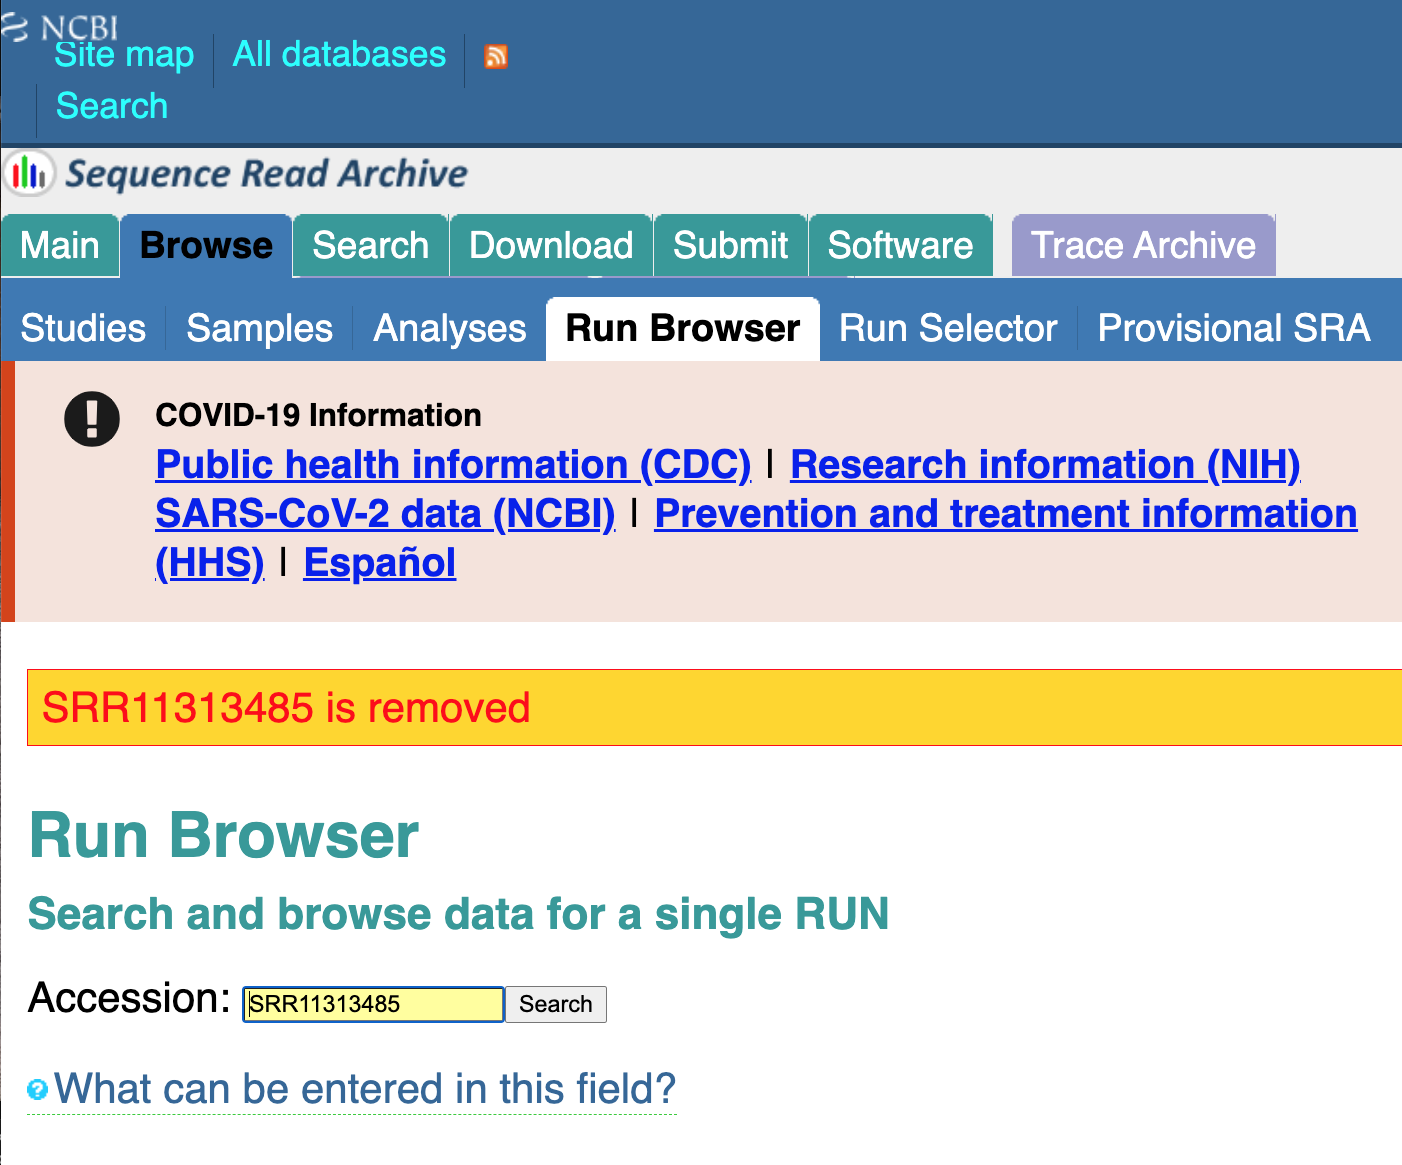
\includegraphics[trim={0.2in 0 0 9in},clip,width=\linewidth]{figures/acc_removed.png}}
\caption{Searching for individual accessions from deleted deep sequencing project PRJNA612766 revealed they had been removed from the SRA.
Shown is the result of searching for ``SRR11313485'' to reach the \url{https://trace.ncbi.nlm.nih.gov/Traces/sra/?run=SRR11313485}.
A copy of this result has been digitally archived on the Wayback Machine at \url{https://web.archive.org/web/20210502131630/https://trace.ncbi.nlm.nih.gov/Traces/sra/?run=SRR11313485}.
}%
\label{fig:acc_removed}
\end{figure}

\subsection{The deleted data set contains sequencing of viral samples collected early in the Wuhan outbreak}

\subsection{Recovery of the data from the Google and Amazon clouds} 

\section{Figures and Tables}

\subsection{Sample Figure}

Figure \ref{fig:spectrum} shows an example figure.

\begin{figure}[htbp!]
\centering
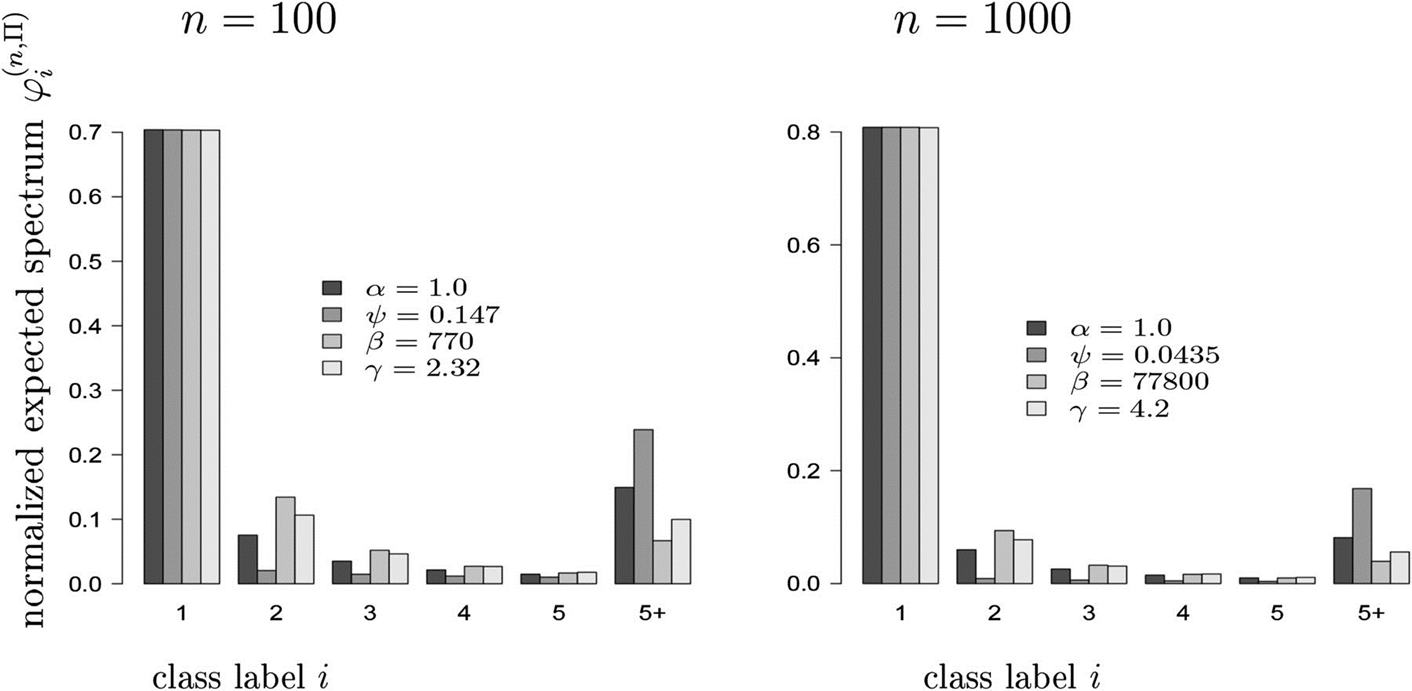
\includegraphics[width=\linewidth]{example-figure}
\caption{captions  
}%
\label{fig:spectrum}
\end{figure}


\subsection{Sample Table}

Table \ref{tab:shape-functions} shows an example table. Avoid shading, color type, line drawings, graphics, or other illustrations within tables. Use tables for data only; present drawings, graphics, and illustrations as separate figures. Histograms should not be used to present data that can be captured easily in text or small tables, as they take up much more space.  

Tables numbers are given in Arabic numerals. Tables should not be numbered 1A, 1B, etc., but if necessary, interior parts of the table can be labeled A, B, etc. for easy reference in the text.  


\begin{table*}[htbp]
\centering
\caption{\bf Students and their grades}
\begin{tableminipage}{\textwidth}
\begin{tabularx}{\textwidth}{XXXX}
\hline
Student & Grade\footnote{This is an example of a footnote in a table. Lowercase, superscript italic letters (a, b, c, etc.) are used by default. You can also use *, **, and *** to indicate conventional levels of statistical significance, explained below the table.} & Rank & Notes \\
\hline
Alice & 82\% & 1 & Performed very well.\\
Bob & 65\% & 3 & Not up to his usual standard.\\
Charlie & 73\% & 2 & A good attempt.\\
\hline
\end{tabularx}
  \label{tab:shape-functions}
\end{tableminipage}
\end{table*}

\bibliography{references}

\end{document}